%%%%%%%%%%%%%%%%%%%%%%%%%%%%%%%%%%%%%%%
% Header                              %
%%%%%%%%%%%%%%%%%%%%%%%%%%%%%%%%%%%%%%%
% 
% Revisions: 2017-12-12 Martin Raedel <martin.raedel@dlr.de>
%                       Initial draft
%               
% Contact:   Martin Raedel,  martin.raedel@dlr.de
%            DLR Composite Structures and Adaptive Systems
%          
%                                 __/|__
%                                /_/_/_/  
%            www.dlr.de/fa/en      |/ DLR
% 
%%%%%%%%%%%%%%%%%%%%%%%%%%%%%%%%%%%%%%%
% Content                             %
%%%%%%%%%%%%%%%%%%%%%%%%%%%%%%%%%%%%%%%

% Figs
\begin{subfigure}{0.32\linewidth}
  % Length
  \setlength{\figwidth}{\linewidth}
  % Figure
  \centering
  \tikzexternalenable
  \tikzsetnextfilename{Exp_RVE_HobbiebrunkenT_woArrow_I}
  %%%%%%%%%%%%%%%%%%%%%%%%%%%%%%%%%%%%%%%
% Header                              %
%%%%%%%%%%%%%%%%%%%%%%%%%%%%%%%%%%%%%%%
% 
% Revisions: 2017-12-12 Martin Raedel <martin.raedel@dlr.de>
%                       Initial draft
%               
% Contact:   Martin Raedel,  martin.raedel@dlr.de
%            DLR Composite Structures and Adaptive Systems
%          
%                                 __/|__
%                                /_/_/_/  
%            www.dlr.de/fa/en      |/ DLR
% 
%%%%%%%%%%%%%%%%%%%%%%%%%%%%%%%%%%%%%%%
% Content                             %
%%%%%%%%%%%%%%%%%%%%%%%%%%%%%%%%%%%%%%%

\begin{tikzpicture}[
  every node/.style={
    font=\figurefontsize,
  }
]
  % External figure
  \node[anchor=south west,inner sep=0] (image) at (0,0) {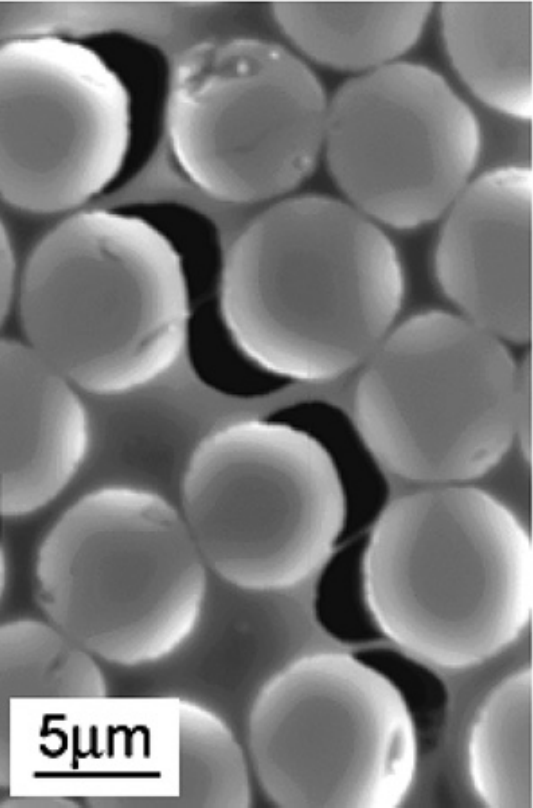
\includegraphics[width=\figwidth,height=\figheight,keepaspectratio]{Exp_RVE_HobbiebrunkenT_woArrow_I}};
  % Figure scope
  \begin{scope}[
    x={(image.south east)},
    y={(image.north west)},
  ]
    % This is influenced by the aspect ratio, but so what
    \coordinate (l1label) at (0.5,0.8);
    \coordinate (l2label) at (0.9,0.828);
    \draw[white,latex-latex] (l1label) -- (l2label) node [midway,below] {Loading};
    
    % Help grid and labels
    %\pic{myimagegrid};
  \end{scope}
\end{tikzpicture}
  \tikzexternaldisable
  \caption{I}%
  \label{fig:Exp:RVE:HobbiebrunkenT:I}
\end{subfigure}%
\hfill
\begin{subfigure}{0.32\linewidth}
  % Length
  \setlength{\figwidth}{\linewidth}
  % Figure
  \centering
  %\tikzexternalenable
  %\tikzsetnextfilename{Obs_Damage_RVE_I_FiberDamage}
  %%%%%%%%%%%%%%%%%%%%%%%%%%%%%%%%%%%%%%%%
% Header                              %
%%%%%%%%%%%%%%%%%%%%%%%%%%%%%%%%%%%%%%%
% 
% Revisions: 2017-12-12 Martin Raedel <martin.raedel@dlr.de>
%                       Initial draft
%               
% Contact:   Martin Raedel,  martin.raedel@dlr.de
%            DLR Composite Structures and Adaptive Systems
%          
%                                 __/|__
%                                /_/_/_/  
%            www.dlr.de/fa/en      |/ DLR
% 
%%%%%%%%%%%%%%%%%%%%%%%%%%%%%%%%%%%%%%%
% Content                             %
%%%%%%%%%%%%%%%%%%%%%%%%%%%%%%%%%%%%%%%

\begin{tikzpicture}[
  every node/.style={font=\figurefontsize},
  %inner sep=0pt,
]
  % External figure
  \node[anchor=south west,inner sep=0] (image) at (0,0) {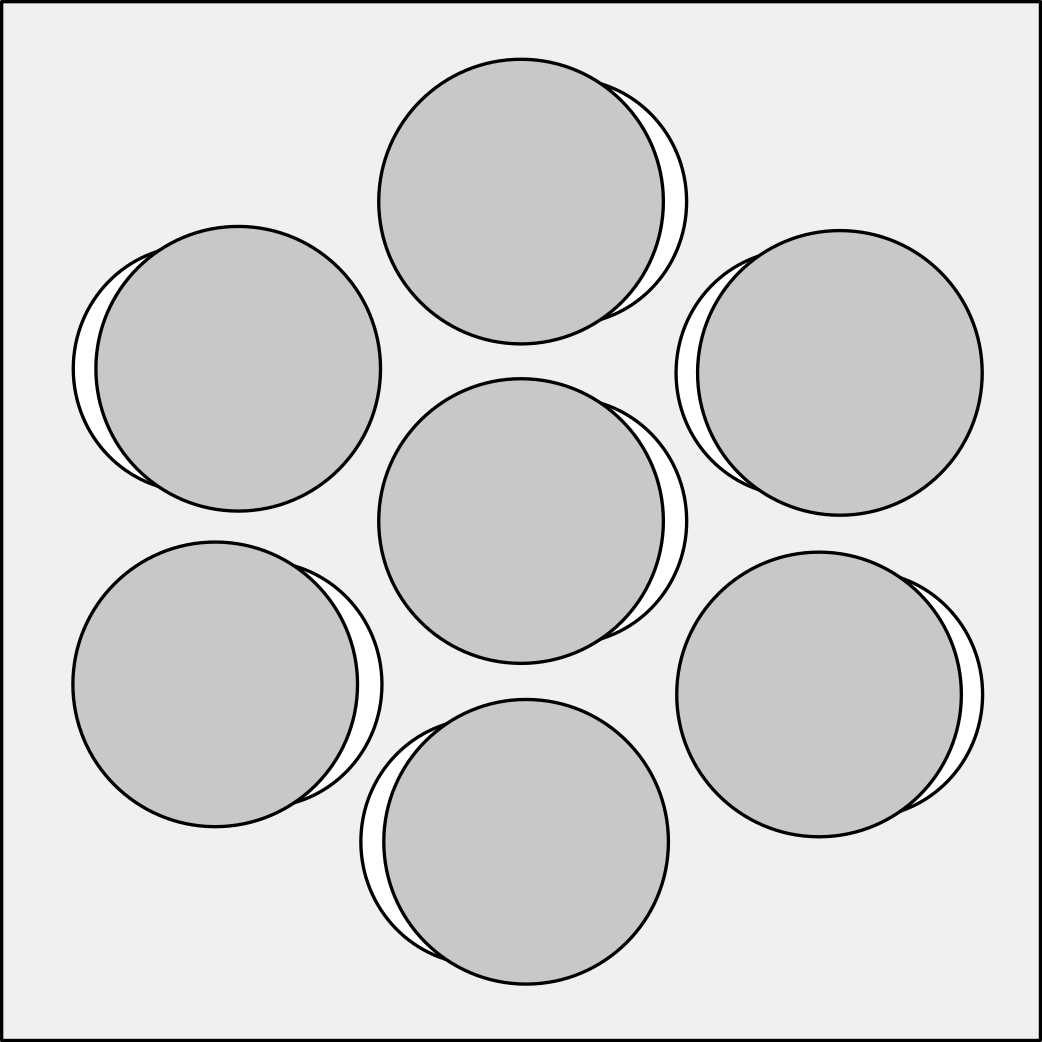
\includegraphics[width=\figwidth]{Obs_Damage_RVE_I_FiberDamage}};
  % Figure scope
  \begin{scope}[
    x={(image.south east)},
    y={(image.north west)},
  ]
    
    % Load arrows
    \foreach \y in {0,1,...,\numarrows} {\draw[-latex] (-0.025,\y/\numarrows) -- (-0.15,\y/\numarrows) coordinate (loadarrowleft\y);}
    \foreach \y in {0,1,...,\numarrows} {\draw[-latex] ( 1.025,\y/\numarrows) -- ( 1.15,\y/\numarrows) coordinate (loadarrowright\y);}
    
    % Help grid and labels
    %\pic{myimagegrid};
  \end{scope}
\end{tikzpicture}
  %\tikzexternaldisable
  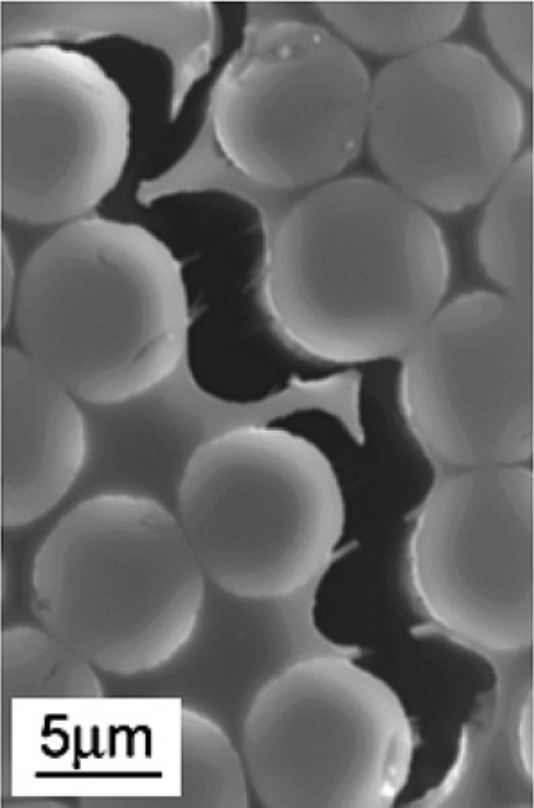
\includegraphics[width=\figwidth,height=\figheight,keepaspectratio]{Exp_RVE_HobbiebrunkenT_woArrow_II}
  \caption{II}%
  \label{fig:Exp:RVE:HobbiebrunkenT:II}
\end{subfigure}%
\hfill
\begin{subfigure}{0.32\linewidth}
  % Length
  \setlength{\figwidth}{\linewidth}
  % Figure
  \centering
  %\tikzexternalenable
  %\tikzsetnextfilename{Obs_Damage_RVE_I_FiberDamage}
  %%%%%%%%%%%%%%%%%%%%%%%%%%%%%%%%%%%%%%%%
% Header                              %
%%%%%%%%%%%%%%%%%%%%%%%%%%%%%%%%%%%%%%%
% 
% Revisions: 2017-12-12 Martin Raedel <martin.raedel@dlr.de>
%                       Initial draft
%               
% Contact:   Martin Raedel,  martin.raedel@dlr.de
%            DLR Composite Structures and Adaptive Systems
%          
%                                 __/|__
%                                /_/_/_/  
%            www.dlr.de/fa/en      |/ DLR
% 
%%%%%%%%%%%%%%%%%%%%%%%%%%%%%%%%%%%%%%%
% Content                             %
%%%%%%%%%%%%%%%%%%%%%%%%%%%%%%%%%%%%%%%

\begin{tikzpicture}[
  every node/.style={font=\figurefontsize},
  %inner sep=0pt,
]
  % External figure
  \node[anchor=south west,inner sep=0] (image) at (0,0) {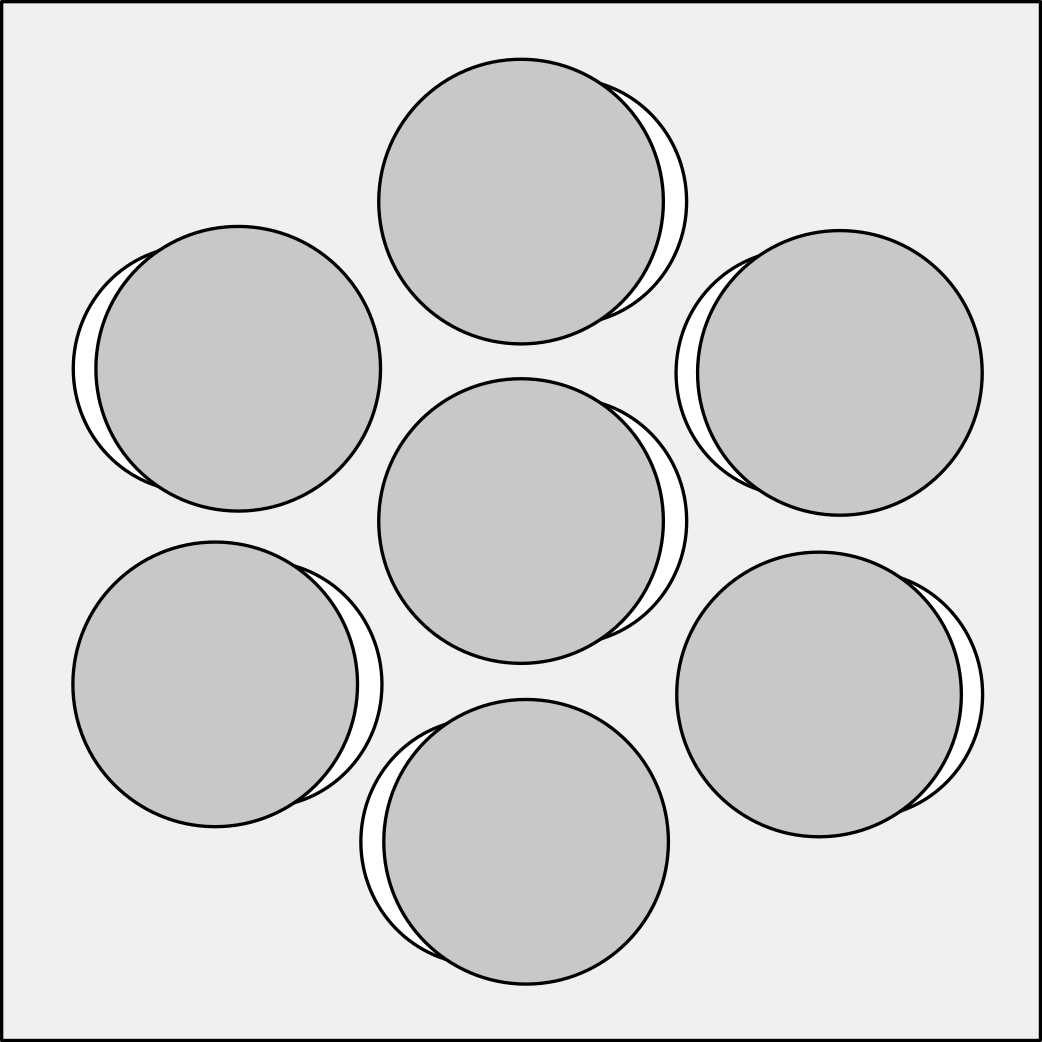
\includegraphics[width=\figwidth]{Obs_Damage_RVE_I_FiberDamage}};
  % Figure scope
  \begin{scope}[
    x={(image.south east)},
    y={(image.north west)},
  ]
    
    % Load arrows
    \foreach \y in {0,1,...,\numarrows} {\draw[-latex] (-0.025,\y/\numarrows) -- (-0.15,\y/\numarrows) coordinate (loadarrowleft\y);}
    \foreach \y in {0,1,...,\numarrows} {\draw[-latex] ( 1.025,\y/\numarrows) -- ( 1.15,\y/\numarrows) coordinate (loadarrowright\y);}
    
    % Help grid and labels
    %\pic{myimagegrid};
  \end{scope}
\end{tikzpicture}
  %\tikzexternaldisable
  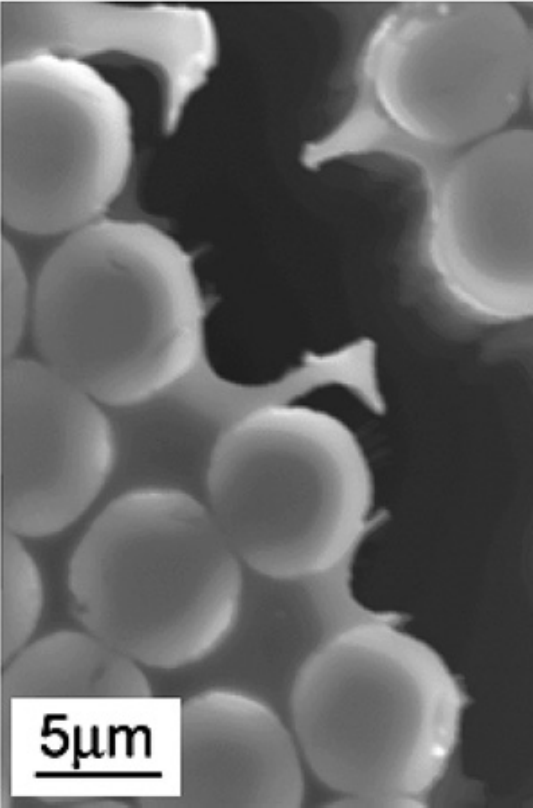
\includegraphics[width=\figwidth,height=\figheight,keepaspectratio]{Exp_RVE_HobbiebrunkenT_woArrow_III}
  \caption{III}%
  \label{fig:Exp:RVE:HobbiebrunkenT:III}
\end{subfigure}%